\documentclass[tikz, border=10pt]{standalone}
\usepackage{tikz}
\usepackage{xcolor}

\usetikzlibrary{shapes, arrows, positioning, fit, calc}

% Define colors
\definecolor{UCMBlue}{RGB}{4, 171, 226}
\definecolor{FixedBlue}{RGB}{20, 65, 134}
\definecolor{AdaptRed}{RGB}{200, 40, 40}
\definecolor{AccentGreen}{RGB}{0, 130, 100}
\definecolor{LightGray}{RGB}{240, 240, 240}

% Define styles
\tikzstyle{block} = [
	draw,
	thick,
	rounded corners=3pt,
	minimum width=1.2cm,
	minimum height=0.6cm,
	font=\tiny,
	align=center
]

\tikzstyle{encoder} = [
	block,
	draw=FixedBlue,
	fill=FixedBlue!20
]

\tikzstyle{decoder} = [
	block,
	draw=AdaptRed,
	fill=AdaptRed!20
]

\tikzstyle{pooling} = [
	block,
	draw=AccentGreen,
	fill=AccentGreen!15
]

\tikzstyle{arrow} = [thick, ->, >=stealth]
\tikzstyle{pool_arrow} = [thick, ->, >=stealth, dashed, color=AccentGreen]
\tikzstyle{indices} = [dashed, thick, <->, color=UCMBlue]

\begin{document}

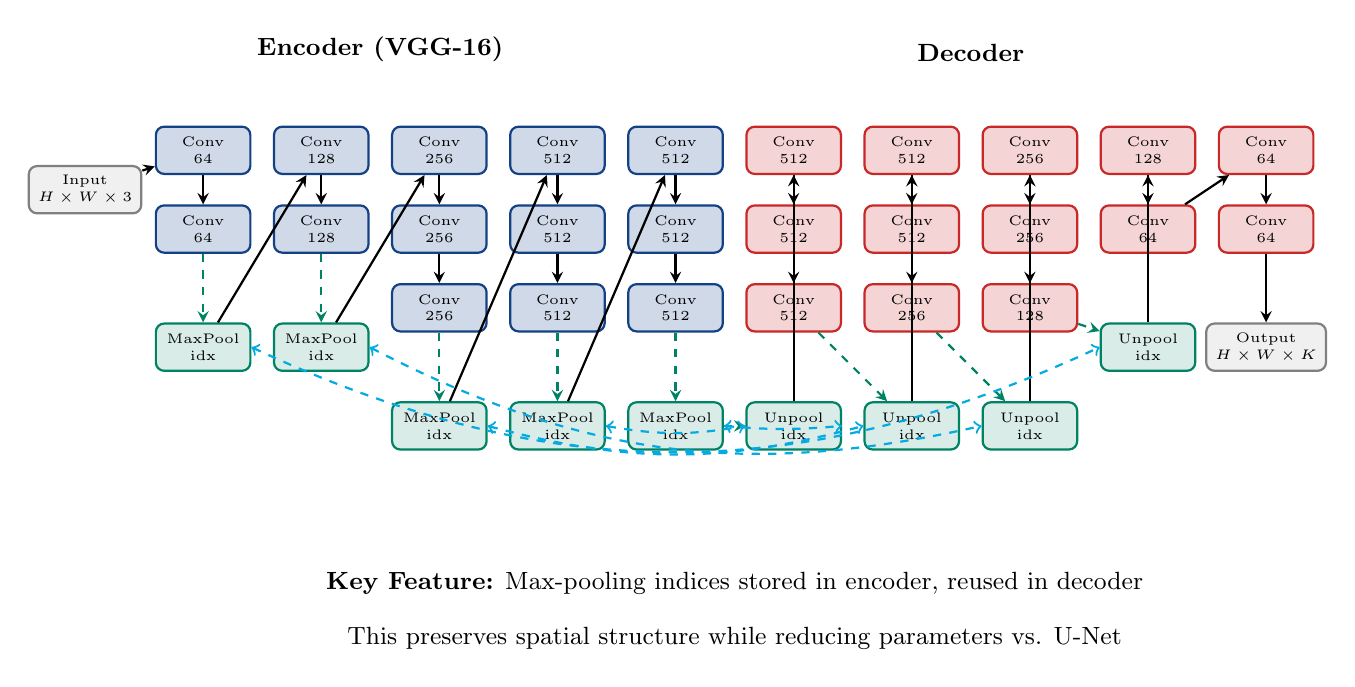
\begin{tikzpicture}[node distance=0.5cm]

	% ========== ENCODER PATHWAY ==========
	% Input
	\node[block, fill=LightGray, draw=gray] (input) at (0, 7) {Input \\ $H \times W \times 3$};

	% Encoder Block 1 (VGG-like)
	\node[encoder] (enc1a) at (1.5, 7.5) {Conv \\ 64};
	\node[encoder] (enc1b) at (1.5, 6.5) {Conv \\ 64};
	\node[pooling] (pool1) at (1.5, 5.0) {MaxPool \\ idx};

	% Encoder Block 2
	\node[encoder] (enc2a) at (3.0, 7.5) {Conv \\ 128};
	\node[encoder] (enc2b) at (3.0, 6.5) {Conv \\ 128};
	\node[pooling] (pool2) at (3.0, 5.0) {MaxPool \\ idx};

	% Encoder Block 3
	\node[encoder] (enc3a) at (4.5, 7.5) {Conv \\ 256};
	\node[encoder] (enc3b) at (4.5, 6.5) {Conv \\ 256};
	\node[encoder] (enc3c) at (4.5, 5.5) {Conv \\ 256};
	\node[pooling] (pool3) at (4.5, 4.0) {MaxPool \\ idx};

	% Encoder Block 4
	\node[encoder] (enc4a) at (6.0, 7.5) {Conv \\ 512};
	\node[encoder] (enc4b) at (6.0, 6.5) {Conv \\ 512};
	\node[encoder] (enc4c) at (6.0, 5.5) {Conv \\ 512};
	\node[pooling] (pool4) at (6.0, 4.0) {MaxPool \\ idx};

	% Encoder Block 5 (final)
	\node[encoder] (enc5a) at (7.5, 7.5) {Conv \\ 512};
	\node[encoder] (enc5b) at (7.5, 6.5) {Conv \\ 512};
	\node[encoder] (enc5c) at (7.5, 5.5) {Conv \\ 512};
	\node[pooling] (pool5) at (7.5, 4.0) {MaxPool \\ idx};

	% ========== DECODER PATHWAY ==========
	% Decoder Block 5
	\node[decoder] (dec5a) at (9.0, 7.5) {Conv \\ 512};
	\node[decoder] (dec5b) at (9.0, 6.5) {Conv \\ 512};
	\node[decoder] (dec5c) at (9.0, 5.5) {Conv \\ 512};
	\node[pooling] (unpool5) at (9.0, 4.0) {Unpool \\ idx};

	% Decoder Block 4
	\node[decoder] (dec4a) at (10.5, 7.5) {Conv \\ 512};
	\node[decoder] (dec4b) at (10.5, 6.5) {Conv \\ 512};
	\node[decoder] (dec4c) at (10.5, 5.5) {Conv \\ 256};
	\node[pooling] (unpool4) at (10.5, 4.0) {Unpool \\ idx};

	% Decoder Block 3
	\node[decoder] (dec3a) at (12.0, 7.5) {Conv \\ 256};
	\node[decoder] (dec3b) at (12.0, 6.5) {Conv \\ 256};
	\node[decoder] (dec3c) at (12.0, 5.5) {Conv \\ 128};
	\node[pooling] (unpool3) at (12.0, 4.0) {Unpool \\ idx};

	% Decoder Block 2
	\node[decoder] (dec2a) at (13.5, 7.5) {Conv \\ 128};
	\node[decoder] (dec2b) at (13.5, 6.5) {Conv \\ 64};
	\node[pooling] (unpool2) at (13.5, 5.0) {Unpool \\ idx};

	% Decoder Block 1
	\node[decoder] (dec1a) at (15.0, 7.5) {Conv \\ 64};
	\node[decoder] (dec1b) at (15.0, 6.5) {Conv \\ 64};

	% Output
	\node[block, fill=LightGray, draw=gray] (output) at (15.0, 5.0) {Output \\ $H \times W \times K$};

	% ========== ENCODER CONNECTIONS ==========
	\draw[arrow] (input) -- (enc1a);
	\draw[arrow] (enc1a) -- (enc1b);
	\draw[pool_arrow] (enc1b) -- (pool1);

	\draw[arrow] (pool1) -- (enc2a);
	\draw[arrow] (enc2a) -- (enc2b);
	\draw[pool_arrow] (enc2b) -- (pool2);

	\draw[arrow] (pool2) -- (enc3a);
	\draw[arrow] (enc3a) -- (enc3b);
	\draw[arrow] (enc3b) -- (enc3c);
	\draw[pool_arrow] (enc3c) -- (pool3);

	\draw[arrow] (pool3) -- (enc4a);
	\draw[arrow] (enc4a) -- (enc4b);
	\draw[arrow] (enc4b) -- (enc4c);
	\draw[pool_arrow] (enc4c) -- (pool4);

	\draw[arrow] (pool4) -- (enc5a);
	\draw[arrow] (enc5a) -- (enc5b);
	\draw[arrow] (enc5b) -- (enc5c);
	\draw[pool_arrow] (enc5c) -- (pool5);

	% ========== DECODER CONNECTIONS ==========
	\draw[pool_arrow] (pool5) -- (unpool5);
	\draw[arrow] (unpool5) -- (dec5a);
	\draw[arrow] (dec5a) -- (dec5b);
	\draw[arrow] (dec5b) -- (dec5c);

	\draw[pool_arrow] (dec5c) -- (unpool4);
	\draw[arrow] (unpool4) -- (dec4a);
	\draw[arrow] (dec4a) -- (dec4b);
	\draw[arrow] (dec4b) -- (dec4c);

	\draw[pool_arrow] (dec4c) -- (unpool3);
	\draw[arrow] (unpool3) -- (dec3a);
	\draw[arrow] (dec3a) -- (dec3b);
	\draw[arrow] (dec3b) -- (dec3c);

	\draw[pool_arrow] (dec3c) -- (unpool2);
	\draw[arrow] (unpool2) -- (dec2a);
	\draw[arrow] (dec2a) -- (dec2b);

	\draw[arrow] (dec2b) -- (dec1a);
	\draw[arrow] (dec1a) -- (dec1b);
	\draw[arrow] (dec1b) -- (output);

	% ========== INDICES CONNECTIONS ==========
	\draw[indices] (pool1.east) to[bend right=25] (unpool2.west);
	\draw[indices] (pool2.east) to[bend right=20] (unpool3.west);
	\draw[indices] (pool3.east) to[bend right=15] (unpool4.west);
	\draw[indices] (pool4.east) to[bend right=10] (unpool5.west);
	\draw[indices] (pool5.east) to[bend right=5] (unpool5.east);

	% ========== SECTION LABELS ==========
	\node[font=\small, anchor=south] at (3.75, 8.5) {\textbf{Encoder (VGG-16)}};
	\node[font=\small, anchor=south] at (11.25, 8.5) {\textbf{Decoder}};

	% ========== LEGEND ==========
	\node[font=\small] at (8.25, 2.0) {\textbf{Key Feature:} Max-pooling indices stored in encoder, reused in decoder};
	\node[font=\small] at (8.25, 1.3) {This preserves spatial structure while reducing parameters vs. U-Net};

\end{tikzpicture}

\end{document}
